\subsection{Nonvalence Anions}

Nonvalence anions are formed when a molecule weakly captures an electron in an extremely diffuse orbital.
It is helpful to further differentiate nonvalence anions due to the dominant mechanism of binding into \gls{nveb} and \gls{nvcb} anions.
\Gls{nveb} anions bind an electron using a permanent electrostatic moment.
For example, an electron can be captured by a molecule or molecular cluster with a sufficiently strong dipole moment, creating a \gls{nveb} anion also called a \gls{dba}.
\Glsxtrlong{nvcb} anions require electron correlation effects to account for the binding of the electron.
This is not to say that the neutral system giving rise to a \gls{nvcb} lacks any permanent electric moments, but rather, that the uncorrelated description of a system containing these permanent moments will not bind the electron.
%The discussion below includes a more detailed description of these systems along with paradigmatic examples.

\subsubsection{Nonvalence Electrostatically Bound Anions}

\Glspl{dba} are formed when a molecule with sufficiently large dipole moments (1.625 D in the Born-Oppenheimer approximation) capture an electron in a diffuse, nonvalence orbital.\cite{10.1063/1.432599,10.1103/PhysRevA.54.1906,10.1063/1.453801,10.1103/PhysRev.72.399,10.1103/PhysRev.174.81,10.1088/0370-1328/91/2/303,10.1016/0009-26147080045-8,10.1103/PhysRevA.3.961,10.1103/PhysRevA.3.961,10.1103/PhysRevLett.73.2436,10.1103/PhysRevLett.73.2436,10.1146/annurev.physchem.54.011002.103851}.
Initially, one may be tempted to think that electron correlation would not play a significant role in such systems given the diffuse nature of the excess electron.
However the excess electron is bound far from the valence electrons, there is a dispersion interaction between the excess electron and the neutral molecule.\cite{10.1021/jp972600z,10.1021/jp980123u}
However, considering the simplified expression for London dispersion it can be seen that the dispersion interaction is dependent on the polarizability of the two interacting entities.\cite{10.1039/TF937330008B}
\begin{equation}
	E_{\mathrm{Disp}} = -\left(\frac{3h}{2R^6}\right) \left(\alpha_i \alpha_j \right) \left(\frac{\nu_k \nu_j}{\nu_k + \nu_j} \right)
\end{equation}
where $\alpha$ is the static polarizability, $\nu$ is the ionization potential, and $R$ is the separation distance.
The diffuse electron is spread over a large volume, and therefore has a large polarizability leading to a large dispersion interaction.

\begin{figure}
    \centering
	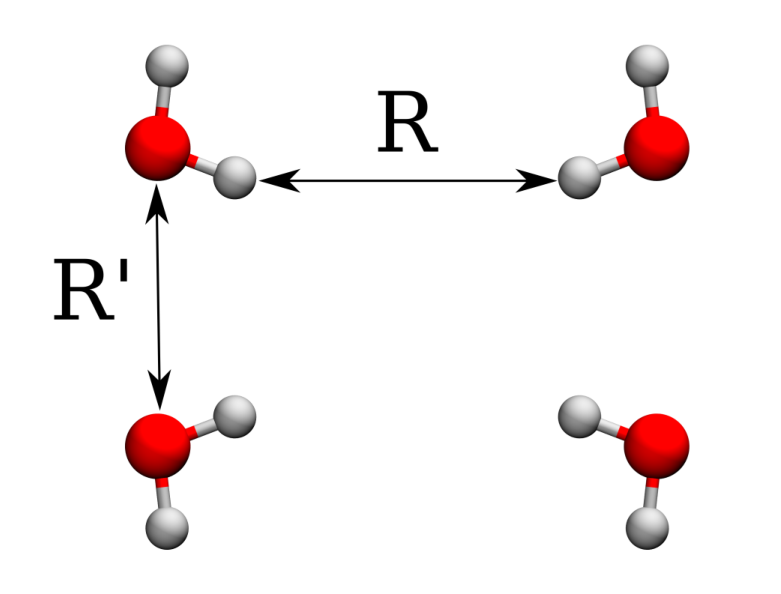
\includegraphics[width=0.9\textwidth,keepaspectratio]{Images/chapter1/h2o4_labeled.eps}
	\caption{A model \ce{(H2O)4} system. The separation between the dimers $R$ is variable, but the separation of two waters within each dimer $r=\SI{2.77514}{\angstrom}$ is fixed.}
	\label{fig:h2o4}
\end{figure}
\Glsxtrlong{nvcb} anions are similar to DBAs, but the leading contribution to the binding energy comes from electronic correlation.
Often this means \gls{nvcb} anions do not posses a dipole moment.
For \glspl{dba}, \glsxtrlong{hf} can bind an electron for molecules with dipole moments above the critical threshold, although the electron would be considerably underbound.
For \gls{nvcb} anions, it has been shown that the \gls{hf} solution is qualitatively incorrect.
Rather than binding the electron, the \gls{hf} solution collapses onto the continuum yielding a wavefunction for the neutral plus an excess electron in a continuum orbital.
When this occurs, methods that build upon the \gls{hf} result such as single reference perturbation theory, or even coupled cluster methods, will also fail to bind the excess electron.
A simple example of this is a model water tetramer cluster that has been studied previously in our group.\cite{10.1063/1.4991497}
This model system can be seen in fig.~\ref{fig:h2o4}.
This system has no dipole moment, and the electron is bound by electrostatics and correlation effects.
By increasing the separation between the two pairs of water dimers, one can induce a crossover from a nonvalence electrostatically-bound anion to a nonvalence \textit{correlation-bound} anion.
\Glspl{dba} can serve as a pathway to valence-bound anions\cite{10.1063/1.475360,10.1063/1.472993,10.1063/1.471484,10.1021/jp9728417}, and nonvalence correlation bound anions can as well.\cite{10.1021/jp408386f}

\begin{figure}
	\centering
	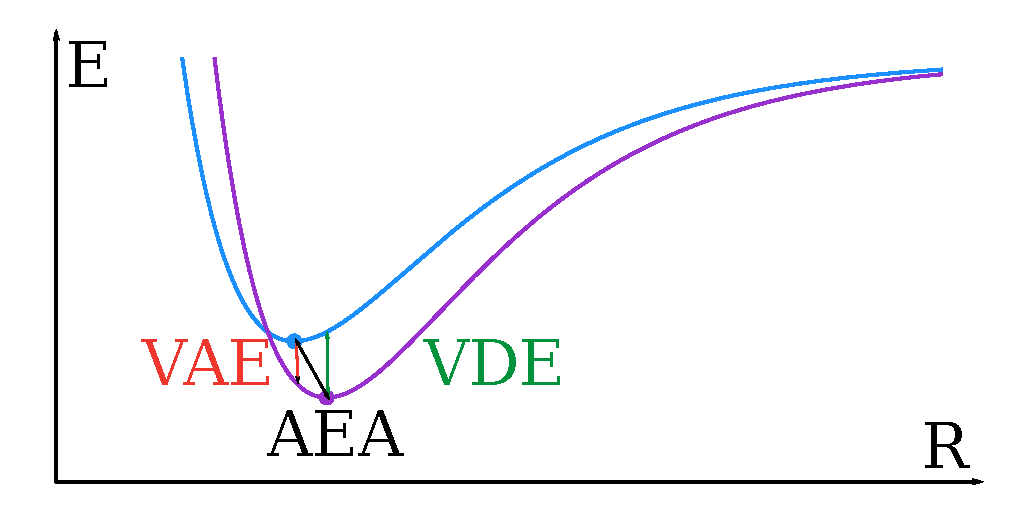
\includegraphics[width=0.9\textwidth,keepaspectratio]{Images/chapter1/morse.eps}
	\caption{Illustrative potential energy curves for a neutral molecule and its corresponding dipole-bound or correlation-bound anion. The energy difference at the neutral geometry is the vertical attachment energy. The energy difference at the anion geometry is the vertical detachment energy. The energy difference between the two respective minima is the \textbf{adiabatic electron affinity}.}
	\label{fig:morse}
\end{figure}

Fig.~\ref{fig:morse} shows illustrative potential energy curves for a hypothetical bound anion.
The coordinate ($R$) represents a collective variable which captures the change in geometry ($\delta R$) that the neutral molecule undergoes upon capturing an electron.
The change in energy associated with binding the electron and the subsequent change in geometry is termed the adiabatic electron affinity.
The change in energy associated only with binding the electron may occur at either the neutral or anionic geometry and is termed the vertical electron affinity and vertical detachment energy respectively.
The extremely diffuse nature of the excess electron in \glspl{dba} and \gls{nvcb} anions often results in a very minor change in geometry.
In the limit of zero change in geometry ($\delta R \rightarrow 0$), the adiabatic electron affinity, vertical electron affinity, vertical detachment energy are equal.
For the \glspl{dba} in this thesis the geometrical distortions are minimal, and therefore it is sufficient to calculate only one of these energies.
In practice, and in this work, it is easiest to calculate the vertical electron affinity as this only requires the ground state neutral geometry.
The magnitude by which the electron is bound is also referred to as the \gls{ebe}.
The sign convention adopted is that a positive \glspl{ebe} indicates that the the electron is bound.
